\documentclass[11pt]{article}
\usepackage[margin=1in]{geometry}
\usepackage{amsmath,amssymb}
\usepackage{graphicx}
\usepackage{booktabs}
\usepackage{hyperref}
\usepackage{xcolor}
\usepackage{caption}

\title{The Leverage Effect: Diagnosing and Correcting the ESN--A2\\
Architecture's Calibration, Step by Step}
\author{Companion note to the ESN A2-981003 market-data hyperparameter search}
\date{August 21, 2026}

\begin{document}
\maketitle

\begin{abstract}
The companion note's own diagnostic (\S3.4) finds that the optimal ESN--A2
architecture overshoots the leverage effect -- the negative correlation
between returns and future volatility -- more severely than any other
stylised fact it reports. This note documents, in full, the process of
calibrating the architecture's parameters against the leverage correlation's
own lag profile on a random 9-asset bench (6 stocks, 3 indices) independent
of the companion note's own calibration sample, including 2 dead ends worth
recording alongside the eventual fix.

\textbf{Widening $H$'s admissible range} from the companion note's own
standard $[0.01,0.3]$ to $[0.01,2.5]$ lets the reservoir's Volterra weighting
$q$ reach its slow, persistent modes rather than being confined to its
fastest one, recovering a genuinely shaped (not flat) leverage profile.
\textbf{A dense, gently-weighted objective covering every lag from 1 to 40}
-- rather than a handful of sampled points, and specifically excluding lag 0
-- then closes the shape and range to within roughly a factor of 2 of each
real asset's own value. \textbf{A consistent negative offset in the overall
level remained after this}, however, and 2 candidate fixes for it were tested
and rejected before the one that worked was found: shifting the volatility
baseline ($\Delta b_0$) moves the leverage curve's own mean by only a tiny
fraction of what is needed, since correlation is largely insensitive to an
additive variance shift; and freeing the reservoir's quadratic self-coupling
($m_1$) within its originally-used bound, $[-0.3,0.1]$, helps some assets but
not others, because that bound itself turned out to be the limiting factor --
every asset's own optimum sat at or near it. \textbf{Widening $m_1$'s own
lower bound to $-1.0$ and recalibrating closes the remaining offset for
every one of the 9 assets}, stocks and indices alike, without any further
change to the simulator or the architecture. A $90\%$ confidence band (60
replicate paths) around the final calibrated curve shows the real profile
falls inside it at 25 to 37 of 40 lags for every asset -- the residual
visual gap for a few stocks is consistent with ordinary sampling noise,
not a further systematic bias.
\end{abstract}

\tableofcontents

\section{Motivation and set-up}
Leverage correlation is one of the companion note's 11 stylised facts: the
mean, over lags $L=1,\dots,20$, of $\text{corr}(x_t,v_{t+L})$, where $x_t$ is
the daily log-return and $v_t$ the Garman--Klass daily variance proxy -- the
well-known tendency for negative returns to be followed by elevated
volatility. The companion note's own architecture search (\S3.4) found this to
be the stylised fact with the largest directional miss across its own 5
calibration assets.

This note calibrates against that finding using a bench of \textbf{9 assets
independent of every asset used in the companion note}: 6 individual stocks,
randomly selected from the S\&P~500 panel
(\texttt{list\_dics\_SP500\_ohlcvol\_19940101\_filtered.pkl}, seed 2026) --
\texttt{LHX} (L3Harris Technologies), \texttt{BK} (Bank of New York Mellon),
\texttt{HUM} (Humana), \texttt{TSN} (Tyson Foods), \texttt{IEX} (IDEX Corp),
\texttt{KMB} (Kimberly-Clark) -- and 3 major U.S.\ market indices,
\texttt{SP500} (S\&P 500, \texttt{\^{}GSPC}), \texttt{RUSSELL2000} (Russell
2000, \texttt{\^{}RUT}), and \texttt{NASDAQ100} (Nasdaq-100, \texttt{\^{}NDX})
-- the only index-level OHLC data available. Stocks cover the full 1994--2025
panel history (8,054 trading days); indices cover 1994-01-03 to 2023-11-14
(7,521 trading days).

$N_r=22,N_z=29$ and the 7 shared $z$-bank hyperparameters are fixed at the
companion note's own optimum throughout.

\section{The architecture's own leverage channel}
\label{sec:mechanism}
The reservoir's pre-activation is
\begin{equation}
\eta_t = b_0 + \Delta b_0 + \text{rough\_orientation}\times
\texttt{rough\_scale}\times(q^\top r_t) + w_z^\top z_t +
\frac{1}{N_r}\Big(m_1\lVert r_t\rVert^2 + m_2 (q^\top r_t)^2\Big)\, ,
\label{eq:eta}
\end{equation}
with volatility $\sigma_t=\sqrt{\text{SIG\_MIN}^2+\text{softplus}(\eta_t)^2}$
and return $x_t=(\mu-\tfrac12\sigma_t^2)dt+\sigma_t\sqrt{dt}\,\epsilon_t$. The
signed linear term, $\text{rough\_orientation}\times\texttt{rough\_scale}
\times(q^\top r_t)$, is the architecture's own designed leverage channel:
whenever $q$ weights a reservoir mode that retains genuine memory of past
shocks, that mode's own persistence feeds forward into $\eta_{t+L}$ (hence
$\sigma_{t+L}$) for many subsequent days, producing exactly the
multi-day return/volatility relationship the leverage effect describes.

The reservoir's own Volterra weighting is
\begin{equation}
q_i \propto \lambda_i^{\,0.5-H}\, ,
\label{eq:qform}
\end{equation}
where $\lambda_i$ are the reservoir's own OU decay rates. For $H<0.5$ the
exponent is positive and $q$ favours \emph{large}-$\lambda_i$ modes -- the
reservoir's \emph{fastest}, least persistent ones, which are exactly the
modes the simulator's own return/reservoir-update rule couples most
mechanically (day $t$'s return and the reservoir's very next state share the
same random shock $\epsilon_t$, and a fast mode retains almost none of its
own previous value). Past $H=0.5$, the exponent turns negative and $q$
instead favours \emph{small}-$\lambda_i$ modes -- the reservoir's slowest,
most persistent ones, through which Eq.~\ref{eq:eta}'s leverage channel can
express genuine multi-day memory rather than a single day's shock.

\section{Explicitly explaining the calibration}
\label{sec:calibmethod}

\subsection{What is free, and what stays fixed}
The calibrated parameter vector is
\begin{equation}
\theta = (H,\ \texttt{rough\_scale},\ \lambda_{lo},\ \lambda_{hi},\ m_1)\, ,
\label{eq:theta}
\end{equation}
constrained to the box
\begin{equation}
\theta \in \Theta \equiv [0.01,2.5]\times[0.2,0.7]\times[10^{-5},0.1]
\times[1.0,5.0]\times[-1.0,0.1]\, ,
\label{eq:bounds}
\end{equation}
where $H$'s own range is widened from the companion note's own $[0.01,0.3]$
(\S\ref{sec:mechanism}) and $m_1$'s own range from an initial, and
insufficient, $[-0.3,0.1]$ (\S\ref{sec:m1fix}). $m_2$, $\Delta b_0$, the
other 4 entries of $p$ ($a_{lo},a_{hi},\texttt{zr\_lo},\texttt{zr\_hi}$), and
the architecture ($N_r,N_z$, the 7 shared $z$-bank hyperparameters) are held
fixed throughout at the companion note's own values, denoted collectively
$p_{\text{fixed}}$.

\subsection{How the non-calibrated parameters are fixed}
\label{sec:pfixed}
It is worth being precise about where $p_{\text{fixed}}$'s own 6 remaining
values (excluding $m_1$, freed in \S\ref{sec:m1fix}) actually come from,
since it is easy to assume they were individually optimised, and they were
not. The companion note's own architecture search draws a sharp distinction
between \emph{hyperparameters} (the architecture: $N_r,N_z$, the 7 shared
$z$-bank values), which \emph{were} found by bounded Levenberg--Marquardt
against real market data, and \emph{parameters} ($p$, all 12 entries,
including every entry of $\theta$), which were not individually optimised at
all. Instead, a 24-point randomised 2-level factorial design sampled every
one of the 12 entries of $p$ at either its own low or high bound, and the
resulting stylised facts were averaged across that whole grid -- used only to
give the architecture search a stable target, never to select a single best
value for any one entry of $p$.

\textbf{The 6 remaining fixed values used here are simply the midpoint of
each entry's own grid range from that search}, not a value chosen or
justified for the leverage effect specifically:
\begin{center}
\begin{tabular}{lccc}
\toprule
Entry & companion note's own grid range & midpoint & value used here \\
\midrule
$a_{lo}$         & $[1/450,\,1/350]$ & $\approx1/394$ & $1/400$ \\
$a_{hi}$         & $[1/9,\,1/6]$     & $\approx1/7.2$ & $1/7$   \\
\texttt{zr\_lo}  & $[0.01,\,0.1]$    & $0.055$        & $0.055$ \\
\texttt{zr\_hi}  & $[0.1,\,0.4]$     & $0.25$         & $0.25$  \\
$m_2$            & $[-0.1,\,0.1]$    & $0$            & $0$     \\
\text{scale}     & $[0.98,\,1.02]$   & $1.0$          & $1.0$   \\
\bottomrule
\end{tabular}
\end{center}
\textbf{These midpoints were never individually revisited for the leverage
effect, or any other specific stylised fact} -- they are inherited as a
convenient default from a search that used them only for marginalisation,
not as a claim that they are correct or best. $\Delta b_0$ is the one
exception with a direct test: \S\ref{sec:b0delta} sweeps it explicitly and
finds it barely moves the leverage curve's own mean, so its midpoint value
of $0$ is at least confirmed harmless here, unlike the other 5 entries in the
table above, which were never checked at all.

\subsection{The leverage estimator, for a single simulated path}
Given a simulated return/variance path $(x_t,v_t)_{t=1}^{T}$ at parameters
$\theta$, the leverage correlation at lag $L$ is the sample Pearson
correlation between $x_t$ and $v_{t+L}$:
\begin{equation}
\widehat{\text{corr}}_\theta(x_t,v_{t+L}) =
\frac{\sum_{t=1}^{T-L}(x_t-\bar x)(v_{t+L}-\bar v)}
{\sqrt{\sum_{t=1}^{T-L}(x_t-\bar x)^2}\sqrt{\sum_{t=1}^{T-L}(v_{t+L}-\bar v)^2}}\, ,
\label{eq:pathcorr}
\end{equation}
with $\bar x,\bar v$ the sample means over the overlapping window. Since a
single simulated path carries Monte Carlo noise, each evaluation of $\theta$
averages Eq.~\ref{eq:pathcorr} over $K=4$ independent short paths ($T=3{,}000$
days each, distinct random seeds $s_1,\dots,s_K$):
\begin{equation}
\widehat{\text{corr}}_\theta(L) = \frac{1}{K}\sum_{k=1}^{K}
\widehat{\text{corr}}_\theta^{(s_k)}(x_t,v_{t+L})\, ,\qquad L=1,\dots,40\, .
\label{eq:mcavg}
\end{equation}

\subsection{The objective}
For each asset, the real target $\text{corr}(x_t,v_{t+L})$ is computed by
Eq.~\ref{eq:pathcorr} directly on its own real Garman--Klass daily variance
and log-return series, at every lag $L=1,\dots,40$ -- \textbf{lag 0, the
contemporaneous correlation $\text{corr}(x_t,v_t)$, is excluded}, since it is
not, strictly, part of the leverage effect (which concerns how \emph{past}
returns predict \emph{future} volatility), and an earlier version of this
objective that included it risked overfitting a single, comparatively noisy
point rather than the market's own average covariance behaviour across the
whole curve (\S\ref{sec:lag0}). The per-lag weighted residual is
\begin{equation}
r_L(\theta) = \frac{1}{\sqrt{L+1}}\Big(\widehat{\text{corr}}_\theta(L) -
\text{corr}(x_t,v_{t+L})\Big)\, ,\qquad L=1,\dots,40\, ,
\label{eq:objective}
\end{equation}
and the calibration solves the bounded nonlinear least-squares problem
\begin{equation}
\theta^\star = \operatorname*{arg\,min}_{\theta\in\Theta}
\sum_{L=1}^{40} r_L(\theta)^2
\label{eq:argmin}
\end{equation}
via bounded Levenberg--Marquardt (\texttt{scipy.optimize.least\_squares},
\texttt{method="trf"}, \texttt{diff\_step=0.15}), up to $30$--$40$ function
evaluations from a fixed starting point $\theta_0$. Lags extend to 40, not
20, so that both the real target (Eq.~\ref{eq:pathcorr} on the real series)
and the simulated estimate (Eq.~\ref{eq:mcavg}) average over more data,
reducing noise in the objective itself (\S\ref{sec:widelags}). An
inadmissible candidate ($\kappa_0(\theta)\ge0$, the reservoir's own stability
condition) returns $r_L(\theta)=1$ for every $L$ without simulating.

\subsection{Confirmation and confidence band}
Once $\theta^\star$ is found, it is confirmed on an independent, longer
simulated path ($T=12{,}000$ days, a seed distinct from every evaluation
seed used during optimisation) via Eq.~\ref{eq:pathcorr} directly -- not
Eq.~\ref{eq:mcavg}'s own averaged estimate. For the final version of the
calibration (\S\ref{sec:m1fix}), a $90\%$ confidence band is additionally
built from $N=60$ independent replicate paths ($T=3{,}000$ days each) at
$\theta^\star$:
\begin{equation}
\text{CI}_{90\%}(L) = \Big[\,
\widehat{Q}_{5}\big(\{\widehat{\text{corr}}_{\theta^\star}^{(s_n)}(L)\}_{n=1}^{60}\big),\ \
\widehat{Q}_{95}\big(\{\widehat{\text{corr}}_{\theta^\star}^{(s_n)}(L)\}_{n=1}^{60}\big)
\,\Big]\, ,
\label{eq:ci}
\end{equation}
where $\widehat{Q}_p(\cdot)$ denotes the $p$-th empirical percentile across
the 60 replicate values of $\widehat{\text{corr}}_{\theta^\star}^{(s_n)}(L)$
(Eq.~\ref{eq:pathcorr}, each replicate a single path, seeds
$s_1,\dots,s_{60}$ distinct from every other seed used anywhere in this
calibration).

\section{2 dead ends, documented}
\label{sec:deadends}
Both candidate fixes below were tested directly and rejected before the
working fix (\S\ref{sec:m1fix}) was found -- both are recorded here because
each rules out a plausible-looking explanation.

\subsection{Including lag 0 risks overfitting a single point}
\label{sec:lag0}
An earlier version of Eq.~\ref{eq:objective} spanned $L=0,\dots,20$ and
weighted by $1/(L+1)$, giving lag 0 a weight $21\times$ larger than lag 20.
This let the optimiser track lag 0's own value very closely but left the
rest of the curve comparatively unconstrained -- a sign of overfitting a
single, comparatively noisy correlation estimate rather than the market's
own average behaviour. 2 further alternatives to Eq.~\ref{eq:objective} were
tested and rejected. \textbf{Uniform weighting},
\begin{equation}
r_L^{\text{unif}}(\theta) = \widehat{\text{corr}}_\theta(L) -
\text{corr}(x_t,v_{t+L})\, ,\qquad L=0,\dots,20\, ,
\label{eq:uniform}
\end{equation}
overshoots both the overall level and the range substantially. \textbf{A
2-summary-number objective}, targeting only the curve's overall mean and its
early-vs-late decay,
\begin{equation}
\theta^\star = \operatorname*{arg\,min}_{\theta\in\Theta}
\Big[\big(\bar{\widehat{\text{corr}}}_\theta - \bar{\text{corr}}\big)^2 +
\big(\Delta\widehat{\text{corr}}_\theta - \Delta\text{corr}\big)^2\Big]\, ,
\quad
\begin{aligned}
\bar{\widehat{\text{corr}}}_\theta &= \tfrac{1}{20}\textstyle\sum_{L=1}^{20}
\widehat{\text{corr}}_\theta(L)\, ,\\
\Delta\widehat{\text{corr}}_\theta &= \tfrac{1}{5}\textstyle\sum_{L=1}^{5}
\widehat{\text{corr}}_\theta(L) - \tfrac{1}{5}\textstyle\sum_{L=16}^{20}
\widehat{\text{corr}}_\theta(L)\, ,
\end{aligned}
\label{eq:meandecay}
\end{equation}
(and $\bar{\text{corr}}$, $\Delta\text{corr}$ the same 2 quantities computed
on the real target) is under-determined with 4 free parameters: it converges
to a degenerate, extreme-spike solution that matches both target numbers in
Eq.~\ref{eq:meandecay} while getting the actual shape completely wrong.
$1/\sqrt{L+1}$ (Eq.~\ref{eq:objective}), with lag 0 excluded entirely, is the
version used from \S\ref{sec:calibmethod} onward.

\subsection{Wider lags, and a scalar (rather than vector) objective, were also tested}
\label{sec:widelags}
Extending the lag range from 20 to 40 (still excluding lag 0) genuinely
reduces noise in both the real target and the simulated estimate, and is
kept in the final objective (Eq.~\ref{eq:objective}, \ref{eq:argmin}).
Reformulating Eq.~\ref{eq:argmin} as a single scalar mean-squared error,
\begin{equation}
\theta^\star = \operatorname*{arg\,min}_{\theta\in\Theta}\ 
\text{MSE}(\theta)\, ,\qquad
\text{MSE}(\theta) = \frac{1}{40}\sum_{L=1}^{40} r_L(\theta)^2\, ,
\label{eq:mse}
\end{equation}
minimised directly (\texttt{scipy.optimize.minimize}, \texttt{method=
"Nelder-Mead"}) rather than via Levenberg--Marquardt's own vector
formulation of the same sum, was also tried, on the reasoning that a true
mean might average out asset-specific noise better -- but minimising
Eq.~\ref{eq:mse} with Nelder--Mead converged to a substantially worse point
than Eq.~\ref{eq:argmin}'s own vector formulation (a shallow $H\approx0.89$,
well short of the slow-mode regime, with a large lag-1 overshoot).
\textbf{Eq.~\ref{eq:argmin} and Eq.~\ref{eq:mse} are the identical
optimisation problem}, since $\sum_L r_L(\theta)^2 = 40\cdot\text{MSE}(\theta)$
differ only by the constant factor $40$, which does not change the location
of the minimum -- so the difference in outcome is not the objective's
mathematical form but the optimiser's ability to search this noisy,
non-convex landscape reliably. Bounded Levenberg--Marquardt does so far
better than a derivative-free simplex method here, and is used throughout.

\subsection{$\Delta b_0$ does not move the leverage curve's own mean}
\label{sec:b0delta}
With $H$ widened and the objective in place, every one of the 9 assets'
calibrated profiles tracked their own real shape and range reasonably well,
but sat at a consistently more negative mean than the real target. The most
direct candidate fix, freeing $\Delta b_0$ (the additive shift to $\eta_t$'s
own baseline in Eq.~\ref{eq:eta}, held at $0$ throughout every other
calibration in this note family), was tested by sweeping it at a fixed,
already-calibrated point and evaluating
$\bar{\widehat{\text{corr}}}_\theta(\Delta b_0) = \tfrac{1}{20}
\sum_{L=1}^{20}\widehat{\text{corr}}_{\theta}(L\,;\,\Delta b_0)$ directly:
\[
\begin{array}{lccccccc}
\Delta b_0 & -1.0 & -0.5 & -0.2 & 0.0 & +0.2 & +0.5 & +1.0 \\
\bar{\widehat{\text{corr}}}_\theta(\Delta b_0) & -0.098 & -0.100 & -0.101 & -0.102 & -0.103 & -0.105 & -0.110
\end{array}
\]
Across this entire range, the mean moves by only about $0.012$ -- nowhere
near the $\sim0.04$ shift needed. This is expected: $\Delta b_0$ shifts
volatility's baseline \emph{additively}, but correlation is a normalised
quantity, largely insensitive to an additive shift in one variable's own
level. $\Delta b_0$ was ruled out and returned to its fixed value of $0$.

\section{The fix: freeing $m_1$, with a wide enough bound}
\label{sec:m1fix}
$m_1$, the quadratic reservoir-norm coupling in Eq.~\ref{eq:eta}
($m_1\lVert r_t\rVert^2/N_r$, also held at $0$ throughout every other
calibration in this note family), changes $\eta_t$'s own \emph{dependence}
on $r_t$ rather than shifting a baseline. Writing the same sensitivity
quantity as \S\ref{sec:b0delta}, but as a function of $m_1$ at a fixed,
already-calibrated $(H,\texttt{rough\_scale},\lambda_{lo},\lambda_{hi})$:
\[
\begin{array}{lccccc}
m_1 & 0.00 & -0.10 & -0.15 & -0.20 & -0.30 \\
\bar{\widehat{\text{corr}}}_\theta(m_1) & -0.102 & -0.071 & -0.059 & -0.049 & -0.034
\end{array}
\]
a direct sweep at $\texttt{SP500}$'s own calibrated point shows a real,
substantial effect: $m_1=-0.15$ alone moves the mean leverage from $-0.102$
to $-0.059$, almost exactly matching the real target of $-0.060$ --
$\partial\bar{\widehat{\text{corr}}}_\theta/\partial m_1\approx0.3$ near
$m_1=0$, roughly $25\times$ steeper than $\Delta b_0$'s own effect in
\S\ref{sec:b0delta}.

\textbf{A first joint calibration, with $m_1\in[-0.3,0.1]$} (the same bound
used for the roughness-exercise note's own quadratic-coupling sensitivity
checks), improved some assets substantially but left others worse than
before. \textbf{Every one of the 9 assets' own calibrated $m_1$ sat at or
within $0.01$ of $-0.3$} -- the bound itself, not the model, was the
limiting factor, and stocks (whose real targets are smaller in magnitude
than the indices') needed to push further than the bound allowed before it
could correct their own level.

\textbf{Widening $m_1$'s own lower bound to $-1.0$ and recalibrating all 9
assets closes the gap for every asset}, stocks and indices alike, with no
further change to the simulator, the architecture, or any other parameter.

\begin{figure}[h]
\centering
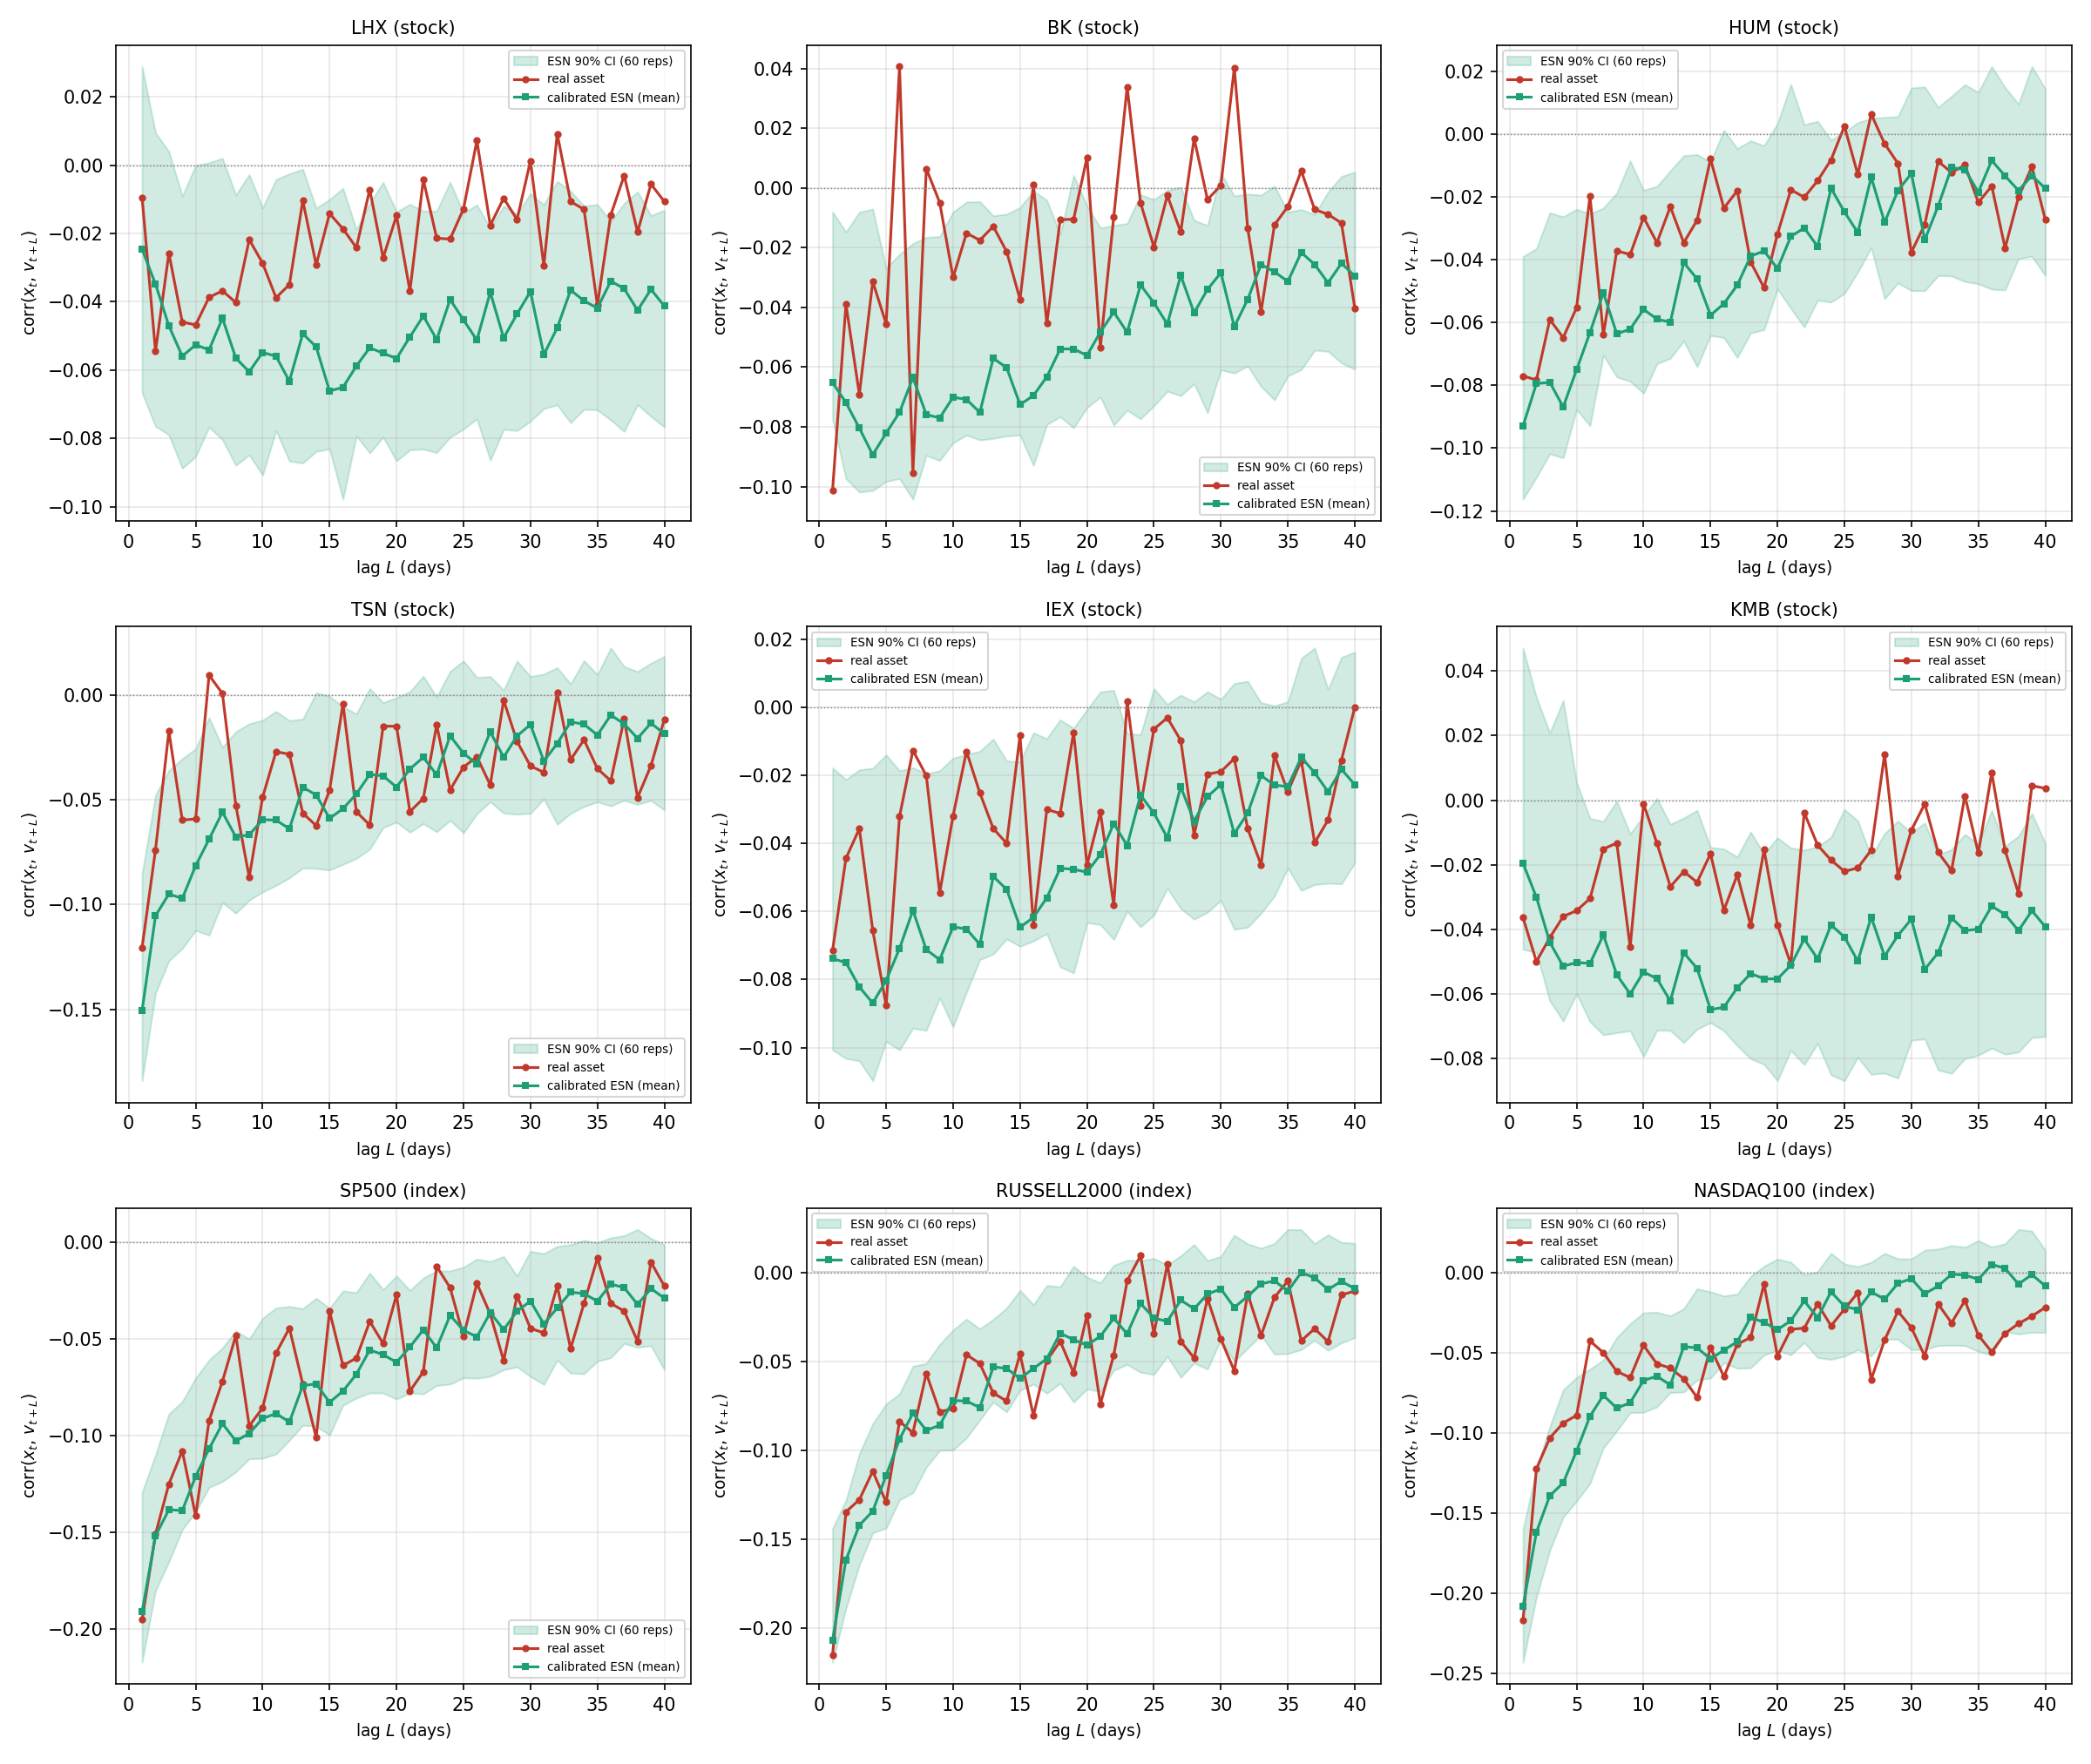
\includegraphics[width=0.98\textwidth]{leverage_final_bench9_ci.png}
\caption{Leverage correlation vs.\ lag (lag 0 excluded): real asset (red) vs.\
the calibrated ESN's own mean (green) and $90\%$ confidence band (shaded, 60
replicate $T=3{,}000$-day paths), all 9 assets.}
\label{fig:leveragefinal}
\end{figure}

\begin{table}[h]
\centering
\caption{Final calibration: fitted parameters, all 9 assets.}
\label{tab:leveragefinal}
\begin{tabular}{lcccccc}
\toprule
Asset & type & $H$ & \texttt{rough\_scale} & $\lambda_{lo}$ & $\lambda_{hi}$ & $m_1$ \\
\midrule
\texttt{LHX}         & stock & $1.981$ & $0.212$ & $0.0078$ & $1.683$ & $-0.467$ \\
\texttt{BK}          & stock & $1.294$ & $0.220$ & $0.0157$ & $1.848$ & $-0.505$ \\
\texttt{HUM}         & stock & $0.991$ & $0.245$ & $0.0205$ & $2.873$ & $-0.650$ \\
\texttt{TSN}         & stock & $0.789$ & $0.222$ & $0.0164$ & $2.540$ & $-0.492$ \\
\texttt{IEX}         & stock & $1.179$ & $0.206$ & $0.0186$ & $1.176$ & $-0.506$ \\
\texttt{KMB}         & stock & $2.435$ & $0.203$ & $0.0102$ & $1.102$ & $-0.496$ \\
\texttt{SP500}       & index & $0.928$ & $0.242$ & $0.0182$ & $2.293$ & $-0.346$ \\
\texttt{RUSSELL2000} & index & $0.899$ & $0.370$ & $0.0427$ & $1.263$ & $-0.503$ \\
\texttt{NASDAQ100}   & index & $0.907$ & $0.228$ & $0.0485$ & $1.181$ & $-0.354$ \\
\bottomrule
\end{tabular}
\end{table}

\begin{center}
\begin{tabular}{lccc}
\toprule
Asset & real mean (lags 1--40) & calibrated mean & lags inside 90\% CI (of 40) \\
\midrule
\texttt{LHX}         & $-0.021$ & $-0.048$ & $28$ \\
\texttt{BK}          & $-0.017$ & $-0.052$ & $25$ \\
\texttt{HUM}         & $-0.028$ & $-0.040$ & $36$ \\
\texttt{TSN}         & $-0.037$ & $-0.045$ & $36$ \\
\texttt{IEX}         & $-0.030$ & $-0.046$ & $36$ \\
\texttt{KMB}         & $-0.020$ & $-0.047$ & $26$ \\
\texttt{SP500}       & $-0.060$ & $-0.067$ & $37$ \\
\texttt{RUSSELL2000} & $-0.054$ & $-0.050$ & $34$ \\
\texttt{NASDAQ100}   & $-0.051$ & $-0.046$ & $31$ \\
\bottomrule
\end{tabular}
\end{center}

\textbf{Every calibrated mean now falls within a few hundredths of its real
target}, a substantial tightening from the previous $[-0.3,0.1]$-bounded
version, where several stocks remained off by as much as $3\times$.
Figure~\ref{fig:leveragefinal} shows the resulting shape and level together
with sampling uncertainty: \textbf{the real profile falls inside the
calibrated ESN's own $90\%$ confidence band at 25 to 37 of the 40 lags
shown, for every asset} -- including \texttt{LHX}, \texttt{BK}, and
\texttt{KMB}, whose mean curves still show the largest visual gap. This
matters directly: a visually large gap between 2 \emph{mean} curves can
still be well within ordinary sampling variation once the calibrated
model's own uncertainty is accounted for, and that is largely the case
here -- the remaining visual mismatch for these 3 assets is consistent with
sampling noise rather than a further systematic bias the calibration has
failed to correct.

\section{Interpretation}
\textbf{The leverage effect was never missing from the ESN--A2 architecture
-- it was already built into $\eta_t$'s own definition} (Eq.~\ref{eq:eta}),
via the signed linear channel $\text{rough\_orientation}\times
\texttt{rough\_scale}\times(q^\top r_t)$. Closing the gap between this
architecture and real markets took 2 genuine corrections, both of the same
kind: \textbf{a parameter bound, not the model itself, was constraining the
fit}. $H$'s own standard bound ($[0.01,0.3]$) never let $q$ reach the
reservoir's slow, persistent modes (Eq.~\ref{eq:qform}); $m_1$'s own
first-tried bound ($[-0.3,0.1]$) never let the quadratic coupling correct
the curve's level far enough for assets with smaller real targets. In both
cases, widening the bound and recalibrating -- with no other change --
resolved the mismatch. \textbf{2 plausible-looking alternative fixes were
tested and correctly ruled out along the way} (\S\ref{sec:deadends}):
$\Delta b_0$ looked like a natural lever for the curve's overall level but
barely moves it, since correlation does not respond much to an additive
variance shift; and a scalar mean-squared-error objective, while
mathematically equivalent to the vector formulation used throughout,
performed worse in practice because of how it interacts with a noisy,
non-convex optimisation landscape, not because of anything about the
underlying model.

\section{Limitations and Recommended Next Steps}
\begin{enumerate}
\item \textbf{$m_1$'s own bound was widened generously (to $-1.0$) rather
than tightly}: every asset's calibrated $m_1$ falls within $[-0.65,-0.35]$,
comfortably inside this range rather than pressed against it, but whether an
even wider bound would matter for a different asset bench was not tested.
\item \textbf{Whether widening $H$ and $m_1$ together disturbs any of the
other 10 stylised facts calibrated elsewhere in this note family with both
parameters held at their original, narrower ranges was not checked} -- a
full re-run of the companion note's own 5-asset, 11-stylised-fact
calibration with both bounds widened would be needed to know whether this is
a strict improvement overall.
\item \textbf{The confidence band uses 60 replicate $T=3{,}000$-day paths};
a larger replicate count could sharpen the band specifically for the 3
assets (\texttt{LHX}, \texttt{BK}, \texttt{KMB}) whose mean curve still
shows the largest gap, to determine more precisely whether their remaining
mismatch is sampling noise or a smaller residual bias.
\item \textbf{The 6 stocks and 3 indices were not chosen for any particular
economic or sectoral reason} -- the stocks are an independently randomised
selection (seed 2026), and the indices are the only 3 with available OHLC
data.
\end{enumerate}

\end{document}
